% Memoria del proyecto de titulación, en formato de congreso IEEE (planificación, sección 6).
% Las cifras salen del README del repositorio, de notebooks/entrenar_tesis.ipynb y de docs/memoria/figuras.py,
% que también genera las dos figuras. Compilar con pdflatex (dos pasadas) o en Overleaf; no usa BibTeX.
% En este computador: & "$env:LOCALAPPDATA\Programs\MiKTeX\miktex\bin\x64\pdflatex.exe" memoria.tex (desde docs/memoria)
\documentclass[conference]{IEEEtran}
\usepackage[utf8]{inputenc}
\usepackage[T1]{fontenc}
\usepackage[spanish,es-tabla,es-nodecimaldot,es-nolayout]{babel}  % sin el diseño español: manda IEEEtran
\usepackage{amsmath}
\usepackage{graphicx}
\usepackage{booktabs}
\usepackage{array}
\usepackage{cite}
\usepackage{url}

\renewcommand{\IEEEkeywordsname}{Palabras clave}
\newcommand{\clase}[1]{\textit{#1}}
\hyphenation{Efficient-Net Res-Net Tensor-Flow}

\begin{document}

\title{Evaluación del compromiso entre desempeño predictivo y eficiencia computacional en la clasificación
automática de muebles de exhibición de punto de venta sobre dispositivos móviles de gama baja}

% Pendiente del autor: correo de contacto y la forma en que el programa pide nombrar al tutor.
\author{\IEEEauthorblockN{Sebastián Garzón}
\IEEEauthorblockA{Maestría en Ciencia de Datos, Colegio de Posgrados\\
Universidad San Francisco de Quito USFQ\\
Quito, Ecuador}
\and
\IEEEauthorblockN{Ricardo Flores Moyano}
\IEEEauthorblockA{Tutor\\
Universidad San Francisco de Quito USFQ\\
Quito, Ecuador}}

\maketitle

\begin{abstract}
Los mercaderistas de Industrias Ales fotografían cada mueble de exhibición contratado en las cadenas de autoservicio
como evidencia del convenio comercial. Este trabajo evalúa si un clasificador de imágenes puede verificar esa
evidencia en el propio teléfono, un Honor X6b de gama baja, sin conexión. Se comparan ResNet-50, MobileNetV3-Large y
EfficientNet-B0, entrenadas por transferencia con 40\,759 fotografías y evaluadas sobre 13\,972 fotografías de 112
locales que los modelos no vieron, en siete clases: cinco tipos de mueble y dos categorías de rechazo.
MobileNetV3-Large alcanza un F1-macro de 0.920 y no difiere de forma significativa de ResNet-50 (0.903), que además
excede el límite de tamaño. La cuantización completa a int8 degrada las arquitecturas eficientes hasta en 0.325 de
F1-macro, mientras que float16 conserva el desempeño con la mitad del tamaño. En el dispositivo, el prototipo
clasifica una fotografía en 71~ms de mediana con 175~MB de memoria pico. Ninguna configuración cumple todos los
criterios de viabilidad fijados de antemano: el recall de captura inválida es 0.644 sobre 90 capturas reales, frente
al 0.90 exigido. Se muestra además que restringir la decisión a los muebles contratados convierte discrepancias en
coincidencias. La decisión se corrige con un umbral calibrado en validación, con el que se detectan 67 de 73
errores reales de campo con 3.0\% de falsas alarmas.
\end{abstract}

\begin{IEEEkeywords}
clasificación de imágenes, aprendizaje por transferencia, cuantización post-entrenamiento, inferencia en el
dispositivo, TensorFlow Lite, retail
\end{IEEEkeywords}

\section{Introducción}

Industrias Ales C.A. fabrica y distribuye productos de consumo masivo en Ecuador y mantiene convenios con cadenas de
autoservicio para instalar muebles de exhibición en sus locales: chicleras, laterales, check outs, cabeceras y
exhibidores de piso. El cumplimiento se verifica en campo. Un equipo de mercaderistas visita cada local y fotografía
cada mueble contratado. Desde septiembre de 2026 ese registro se hace con ODK Collect~\cite{hartung2010odk}, una
aplicación de levantamiento de datos que opera sin conexión: el mercaderista elige el local, el formulario despliega
los muebles con convenio vigente y, sobre cada fila, se adjunta la fotografía.

El punto débil del proceso es esa asociación entre la fotografía y el mueble declarado. La fotografía puede
adjuntarse a una fila que no corresponde, o puede no servir como evidencia: estar oscura, movida o dirigida al piso,
o mostrar algo que no es un mueble. Hoy el error llega a los tableros de cumplimiento sin ningún control, y cuando
se detecta el mercaderista ya no está en la tienda.

Este trabajo propone verificar la fotografía en el propio teléfono, inmediatamente después de la captura, y evalúa
si esa verificación es viable en el equipo que la operación ya usa: un Honor X6b de gama baja, sin unidad de
procesamiento neuronal. El estudio se organiza alrededor de tres preguntas:

\begin{enumerate}
\item ¿Qué diferencia de desempeño predictivo existe entre una arquitectura profunda convencional y arquitecturas
diseñadas para eficiencia, sobre fotografías tomadas en condiciones reales de punto de venta?
\item ¿Cuánto desempeño se pierde y cuánta latencia, memoria y tamaño se ganan con la cuantización
post-entrenamiento a int8 en el dispositivo de referencia?
\item ¿Qué configuraciones de arquitectura y compresión satisfacen a la vez los umbrales operativos definidos, y
cuál ofrece el mejor compromiso?
\end{enumerate}

Los umbrales se fijaron antes de entrenar, en la planificación aprobada del proyecto, junto con la regla para elegir
entre configuraciones viables. Las contribuciones son cuatro: un conjunto de 68\,254 fotografías etiquetadas, con
una partición por local que controla la fuga de información; la comparación de tres arquitecturas y cinco formatos
de despliegue contra esos umbrales; la medición de latencia y memoria en el teléfono real, con un prototipo
integrado al formulario de ODK; y el análisis de la decisión de verificación contra el convenio, que identifica y
corrige una falla del mecanismo previsto.

El resultado principal es negativo y se reporta como tal: ninguna configuración cumple todos los criterios, porque
ninguna arquitectura reconoce suficientes capturas inválidas reales. Los demás criterios, incluidos los del
dispositivo, se cumplen con holgura en las dos arquitecturas eficientes.

\section{Estado del arte}

El reconocimiento visual aplicado a retail se ha concentrado en el producto individual. Tonioni
\textit{et~al.}~\cite{tonioni2018} proponen una tubería de detección y emparejamiento por similitud para productos
en percha. Wei \textit{et~al.}~\cite{wei2019rpc} publican RPC, un conjunto a gran escala para checkout automático.
Goldman \textit{et~al.}~\cite{goldman2019} abordan la detección en escenas densamente pobladas, y Peng
\textit{et~al.}~\cite{peng2020rp2k} presentan RP2K para clasificación de grano fino sobre miles de referencias. La
revisión de Wei \textit{et~al.}~\cite{wei2020review} sistematiza los retos del dominio: similitud entre empaques,
cambios de diseño, oclusiones, reflejos y variabilidad de captura.

En paralelo, la investigación sobre modelos eficientes ha producido arquitecturas diseñadas para el compromiso entre
exactitud y costo. MobileNetV2 introduce los bloques residuales invertidos~\cite{sandler2018}; MobileNetV3 refina
el diseño con búsqueda de arquitectura~\cite{howard2019}; EfficientNet formaliza el escalamiento
compuesto~\cite{tan2019} y EfficientNetV2 optimiza la velocidad de entrenamiento~\cite{tan2021}. Trabajos más
recientes desplazan el criterio de diseño hacia la latencia medida en el dispositivo:
MobileOne~\cite{vasu2023}, MobileViT~\cite{mehta2022} y MobileNetV4~\cite{qin2024}. Sobre compresión, Jacob
\textit{et~al.}~\cite{jacob2018} establecen la cuantización a aritmética entera, Gholami
\textit{et~al.}~\cite{gholami2021} revisan el campo y Hinton \textit{et~al.}~\cite{hinton2015} formulan la
destilación de conocimiento.

La limitación que este trabajo aborda está en la intersección de las dos líneas. Los trabajos de retail toman como
unidad el producto y evalúan en servidor, sin restricciones de despliegue; el mueble de exhibición como objeto a
clasificar y la validación de una evidencia contra una declaración administrativa no aparecen en esa literatura.
Los trabajos de eficiencia reportan latencia en equipos de gama media o alta y sobre conjuntos de referencia, no
sobre un dominio industrial con desbalance severo y un dispositivo de gama baja fijado por la operación.

\section{Descripción de la propuesta}

\subsection{Tarea y taxonomía}

El problema se formula como clasificación de imagen completa, de etiqueta única, en siete categorías. Cinco son
tipos de mueble: \clase{chiclera}, \clase{lateral}, \clase{check out}, \clase{cabecera} y \clase{exhibidor de piso}.
Resultan de consolidar las nomenclaturas de las maestras de convenios, con dos criterios: que las denominaciones
agrupadas correspondan al mismo mueble físico y que las clases se distingan en una fotografía. El tipo de mueble es
la variable adecuada porque se mantiene estable aunque cambien el negocio, la categoría y las marcas que lo ocupan.

Las otras dos son categorías de rechazo, que no existen en la nomenclatura comercial pero son necesarias en
operación. \clase{Captura inválida} es una imagen que no permite identificar ningún mueble por razones técnicas o de
encuadre: oscura, negra, desenfocada, movida, o dirigida al piso o al techo. \clase{Contenido ajeno} es una imagen
legible que muestra otra cosa: la percha regular, producto suelto, personas o pantallas. El alcance es el canal
moderno de autoservicios; farmacias y canal tradicional quedan fuera.

\subsection{Conjunto de datos}

Se usan dos corpus. El histórico reúne las fotografías de 2024 y 2025, anteriores a ODK, que los mercaderistas
subieron sin clasificar a un repositorio corporativo desde cinco cadenas. El de ODK reúne las fotografías de los
formularios en uso desde septiembre de 2026; en el formulario de muebles cada una trae el mueble que el
mercaderista declaró. Las dos fuentes se capturan con la misma aplicación de cámara, que estampa fecha, hora y
local en la esquina inferior derecha.

Ninguna fotografía traía etiqueta. La planificación preveía propagar etiquetas débiles desde la maestra de
convenios~\cite{northcutt2021} y verificar a mano unas 6\,000 imágenes. Se descartó: todas las fotografías se
revisaron a mano, en una herramienta propia que presenta páginas de 24 fotografías con una clase sugerida por un
clasificador auxiliar, independiente de los modelos evaluados. Tras la revisión y la deduplicación, el conjunto
tiene 68\,254 fotografías de 563 locales: 55\,338 del histórico, 10\,830 de ODK y 2\,086 capturas inválidas
sintéticas.

\textbf{Capturas inválidas.} Los mercaderistas están entrenados para no tomarlas, y el histórico aporta dos. Las
276 reales del conjunto vienen de tres fuentes: las que la revisión manual encontró en formularios de ODK, un
formulario en que se pidió a los mercaderistas tomar fotografías malas, y 53 que se tomaron a propósito para este
trabajo en dos locales. Las dos últimas son capturas inducidas y la primera, espontáneas; la
sección~\ref{sec:invalidas} separa sus resultados. Las sintéticas se generan degradando fotografías válidas
(oscuridad con ruido, desenfoque de disco y movimiento) y solo entran al entrenamiento.

\textbf{Control de calidad.} Con la partición ya congelada y antes de tener resultados, una segunda persona
clasificó a ciegas 756 fotografías de validación y prueba, incluidas todas las capturas inválidas. La concordancia
es 0.960, con intervalo de Wilson~\cite{wilson1927} al 95\% de [0.944, 0.972], y el kappa de
Cohen~\cite{cohen1960} es 0.953. De los 30 desacuerdos, 13 son entre las dos categorías de rechazo. No se
arbitraron ni se corrigieron, porque la partición ya estaba congelada; en su lugar se mide cuánto pesan en los
resultados.

\subsection{Partición y control de fuga}

Un mismo local se fotografía cada mes, de modo que partir por fotografía pondría el mismo mueble, con el mismo
fondo, en entrenamiento y en prueba~\cite{kapoor2023}. La partición se hace por local: 401 de entrenamiento, 50 de
validación y 112 de prueba, estratificados por clase. Antes del sorteo se eliminan los cuasi-duplicados dentro de
cada local (distancia de Hamming de hasta 4 entre huellas perceptuales) y las 672 fotografías archivadas en más de
un local, porque no se sabe a cuál pertenecen. La validación y la prueba solo tienen fotografías
verificadas a mano y reales. La lista de fotografías de cada partición se congeló con una huella SHA-256 antes de
entrenar, y el código de entrenamiento la lee sin volver a sortear. Tres locales se asignaron a la prueba por
diseño, porque en ellos se tomaron capturas inválidas para evaluar.

El experimento A mide la generalización a locales no vistos y es el principal. El experimento B mide la
generalización temporal: entrena con las fotografías hasta septiembre de 2025 y evalúa con las de octubre a
diciembre de 2025 de los locales de prueba. La tabla~\ref{tab:datos} muestra la composición del experimento A. El
entrenamiento limita a 300 las fotografías por local, para que los locales más fotografiados no dominen; el tope
deja fuera 6\,359 de las 47\,118 fotografías de los locales de entrenamiento.

\begin{table}[t]
\caption{Fotografías del experimento A por partición, y precisión y recall de MobileNetV3-Large en float16 sobre la
prueba}
\label{tab:datos}
\centering
\setlength{\tabcolsep}{3.5pt}
\begin{tabular}{@{}lrrrcc@{}}
\toprule
Clase & Entren. & Valid. & Prueba & Precisión & Recall \\
\midrule
Chiclera & 5\,355 & 786 & 1\,551 & 0.986 & 0.986 \\
Lateral & 2\,016 & 300 & 634 & 0.935 & 0.845 \\
Check out & 19\,340 & 3\,418 & 7\,354 & 0.993 & 0.977 \\
Cabecera & 3\,831 & 663 & 1\,470 & 0.883 & 0.989 \\
Exhibidor de piso & 4\,665 & 725 & 1\,547 & 0.904 & 0.918 \\
Captura inválida & 1\,586 & 16 & 90 & 0.967 & 0.644 \\
Contenido ajeno & 3\,966 & 618 & 1\,326 & 0.958 & 0.965 \\
\midrule
Total & 40\,759 & 6\,526 & 13\,972 & & \\
\bottomrule
\end{tabular}
\\[2pt]
\footnotesize De las 1\,586 capturas inválidas de entrenamiento, 163 son reales y 1\,423 sintéticas.
\end{table}

\subsection{Criterios de viabilidad}

Una configuración, es decir, una arquitectura en un formato de despliegue, es viable si cumple a la vez los nueve
criterios de la tabla~\ref{tab:criterios}. Se fijaron antes de entrenar. Los predictivos responden al costo del
error: una evidencia inservible que llega al tablero degrada la información, mientras que una alerta injustificada
solo obliga a repetir una fotografía, pero con 20 a 30 fotografías diarias por persona una tasa alta de falsas
alarmas volvería inutilizable la herramienta. Los de eficiencia responden al presupuesto del teléfono, que
comparte memoria con la aplicación de levantamiento y la cámara. Entre configuraciones viables, la regla prevista
es lexicográfica: mayor F1-macro, luego menor latencia p95 y luego menor memoria. Si ninguna es viable, no se
recomienda ninguna y se reporta qué criterio lo impide.

\begin{table}[t]
\caption{Criterios de viabilidad fijados en la planificación}
\label{tab:criterios}
\centering
\begin{tabular}{@{}ll@{}}
\toprule
Criterio & Umbral \\
\midrule
F1-macro sobre la prueba & $\geq 0.85$ \\
Recall-macro & $\geq 0.90$ \\
Recall de cada categoría de rechazo & $\geq 0.90$ \\
Falsas alarmas sobre pares correctos & $\leq 5\%$ \\
Degradación por cuantización & $\leq 0.02$ de F1-macro \\
Latencia mediana en el dispositivo & $\leq 2\,000$~ms \\
Latencia p95 en el dispositivo & $\leq 3\,000$~ms \\
Memoria pico en inferencia & $\leq 300$~MB \\
Tamaño del modelo & $\leq 20$~MB \\
\bottomrule
\end{tabular}
\end{table}

\subsection{Verificación contra el convenio}
\label{sec:decision}

La verificación compara lo que el modelo ve con el mueble declarado y alerta cuando no coinciden o cuando la
fotografía es de rechazo. El convenio de cada local se toma de dos maestras de muebles de Industrias Ales, de junio
de 2025 y de noviembre de 2026, y no de las etiquetas de las fotografías. Cada maestra rige las fotografías tomadas
a menos de seis meses de su fecha. Las maestras listan los muebles alquilados; los ganados en negociación no
figuran, así que un local puede tener muebles que su convenio no trae.

La planificación preveía restringir la predicción a los muebles del convenio más las dos categorías de rechazo.
Esa restricción tiene una falla: si la fotografía muestra un mueble que el convenio no lista, la predicción solo
puede caer en uno contratado, y la discrepancia se convierte en coincidencia. La decisión que se adopta conserva
la clase más probable $c^*$ cuando es un rechazo, un mueble del convenio, o un mueble fuera del convenio con
probabilidad $p(c^*) \geq \tau$. Solo si esa evidencia no alcanza se decide dentro del convenio. El umbral $\tau$
se calibra con la validación de cada red: es el que maximiza la detección de un mueble fuera del convenio menos
las falsas alarmas, es decir, el índice de Youden~\cite{youden1950}. La prueba no interviene en el umbral, pero sí
en el origen de la regla: la falla de la restricción se identificó al analizar los resultados de la prueba, y la
regla se introdujo después, como corrección durante el análisis experimental. Sus resultados en la prueba son
reproducibles, pero no constituyen una estimación independiente.

La verificación se evalúa con dos experimentos que no miden lo mismo. En los \emph{pares por intercambio}, cada
fotografía histórica de un mueble del convenio se declara como cada mueble del local: declararla como otro es una
discrepancia construida, y como lo que es, un par correcto. Sobre estos pares se mide la tasa de falsas alarmas
del criterio de viabilidad. En las \emph{declaraciones reales de ODK}, cada fotografía se evalúa con el mueble que
el mercaderista declaró, de modo que las discrepancias son errores reales de campo.

\section{Desarrollo}

\subsection{Entrenamiento}

Se entrenan tres arquitecturas con pesos preentrenados en ImageNet~\cite{deng2009}: ResNet-50~\cite{he2016} como
línea base sin restricción de eficiencia, y MobileNetV3-Large~\cite{howard2019} y
EfficientNet-B0~\cite{tan2019} como arquitecturas eficientes. El protocolo es común. La entrada es de
$224 \times 224$ píxeles. Toda la red se ajusta, con \emph{dropout} de 0.2 y una capa densa de siete salidas
sobre el promedio global; optimizador Adam con tasa de aprendizaje de $10^{-4}$, lotes de 32, pesos de clase
balanceados, reducción de la tasa cuando la pérdida de validación se estanca y parada temprana con paciencia de
seis épocas. Los aumentos reproducen condiciones de captura: rotación leve, recorte, traslación, brillo y
contraste de hasta 25\%, y compresión JPEG.

La superposición de la cámara incluye el nombre del local, que delata la clase a través del convenio. Se
enmascara dentro del modelo: la región inferior derecha, de 0.70 del ancho por 0.33 del alto, se pone en cero. Como
control se entrena MobileNetV3-Large sin máscara. Las siete corridas (tres arquitecturas en A y en B, y el control)
tomaron 5.3~h en una GPU L4.

\subsection{Formatos de despliegue}

Cada modelo se convierte a TensorFlow Lite~\cite{tflite2022} en cinco formatos: float32; float16, con pesos de
media precisión; int8 de rango dinámico, con pesos enteros y activaciones en coma flotante; int8 completo, con
pesos y activaciones enteros, calibrado con 300 fotografías de entrenamiento al azar; e int8 completo calibrado con
100 fotografías por clase. El int8 completo es el que exige el objetivo; los demás se evalúan para entender dónde
se pierde la exactitud.

\subsection{Medición en el dispositivo}

El dispositivo de referencia es el Honor X6b de la flota corporativa, con procesador MediaTek Helio G85 y 6~GB de
memoria. No tiene unidad de procesamiento neuronal, así que la inferencia corre en la CPU, con XNNPACK. Se mide de
dos formas, en modo avión, con ODK Collect abierto y la pantalla encendida. El modelo solo se mide con la
herramienta de referencia de TensorFlow Lite. El prototipo se mide de extremo a extremo, desde que la fotografía
está en disco hasta la decisión, con fotografías reales. En los dos casos se hacen cuatro ráfagas de 30
inferencias, que concentran en minutos la carga de un día, y se reporta el mayor p95 de las cuatro.

\subsection{Prototipo}

El prototipo es una aplicación Android cuya única dependencia es el intérprete de TensorFlow Lite. Repite el
preprocesamiento del entrenamiento: endereza la fotografía según su orientación EXIF, la reduce a 320 píxeles de
lado mayor y luego a $224 \times 224$. Se integra al formulario de ODK como aplicación externa de la pregunta de
fotografía: recibe el mueble declarado y los muebles del local, abre la cámara, clasifica y devuelve la
fotografía. Sin alerta, la fotografía vuelve sola al formulario; con alerta, la persona decide si la repite o la
usa de todos modos.

\section{Experimentos y análisis de resultados}

\subsection{Desempeño predictivo}

La tabla~\ref{tab:formatos} reúne los resultados sobre las 13\,972 fotografías de prueba. En float32,
MobileNetV3-Large alcanza un F1-macro de 0.920 y EfficientNet-B0, de 0.919; ResNet-50 queda en 0.903. La
diferencia entre ResNet-50 y MobileNetV3-Large es $-0.017$, con intervalo de confianza al 95\% de
$[-0.039, +0.011]$ por bootstrap~\cite{efron1979} que remuestrea locales: la línea base no supera a la arquitectura
eficiente. Además incumple el recall-macro (0.884) y pesa 23~MB en su formato más chico. El control sin máscara
obtiene 0.929, de modo que la superposición aporta cerca de un punto de F1-macro que el modelo desplegado no debe
usar.

Por clase (tabla~\ref{tab:datos} y figura~\ref{fig:confusion}), el mueble más difícil es el lateral, con recall de
0.845: uno de cada diez sale como exhibidor de piso. Los otros cuatro muebles están entre 0.918 y 0.989. El
contenido ajeno se reconoce con recall de 0.965. La clase que falla es la captura inválida.

\begin{figure}[t]
\centering
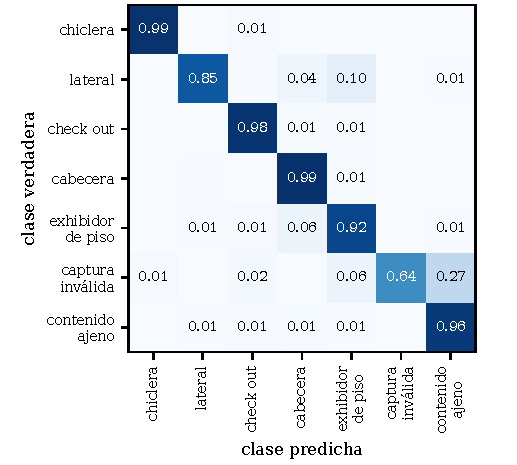
\includegraphics[width=\columnwidth]{fig/confusion.pdf}
\caption{Matriz de confusión de MobileNetV3-Large en float16 sobre la prueba, normalizada por fila.}
\label{fig:confusion}
\end{figure}

\begin{table*}[t]
\caption{Resultados por arquitectura y formato sobre la prueba del experimento A, y medición del modelo solo en el
Honor X6b}
\label{tab:formatos}
\centering
\begin{tabular}{@{}llrcccccrrr@{}}
\toprule
Arquitectura & Formato & MB & F1-macro & Recall-macro & Recall de & Falsas & Caída de & p50 & p95 & Memoria \\
 & & & & & rechazo & alarmas & F1-macro & (ms) & (ms) & (MB) \\
\midrule
MobileNetV3-Large & float32 & 12.4 & 0.920 & 0.903 & 0.644 & 1.5\% & -- & 19 & 22 & 44 \\
 & float16 & 5.9 & 0.920 & 0.903 & 0.644 & 1.5\% & 0.000 & 19 & 25 & 39 \\
 & int8 dinámico & 3.3 & 0.918 & 0.899 & 0.622 & 1.5\% & 0.002 & 23 & 28 & 29 \\
 & int8 completo & 3.4 & 0.594 & 0.617 & 0.211 & 37.6\% & 0.325 & 38 & 45 & 20 \\
\midrule
EfficientNet-B0 & float32 & 16.6 & 0.919 & 0.905 & 0.533 & 1.6\% & -- & 51 & 58 & 66 \\
 & float16 & 7.9 & 0.919 & 0.905 & 0.533 & 1.6\% & 0.000 & 49 & 58 & 90 \\
 & int8 dinámico & 4.6 & 0.920 & 0.908 & 0.556 & 1.6\% & $-0.001$ & 57 & 73 & 44 \\
 & int8 completo & 4.8 & 0.839 & 0.831 & 0.611 & 4.4\% & 0.081 & 22 & 27 & 31 \\
\midrule
ResNet-50 & float32 & 91.0 & 0.903 & 0.884 & 0.489 & 2.0\% & -- & 219 & 228 & 220 \\
 & float16 & 45.0 & 0.903 & 0.884 & 0.489 & 2.0\% & 0.000 & 221 & 230 & 175 \\
 & int8 dinámico & 23.0 & 0.907 & 0.889 & 0.522 & 2.0\% & $-0.004$ & 106 & 111 & 81 \\
 & int8 completo & 23.2 & 0.902 & 0.884 & 0.489 & 2.0\% & 0.001 & 76 & 83 & 72 \\
\bottomrule
\end{tabular}
\\[2pt]
\footnotesize El recall de rechazo es el menor de los dos; en todas las filas es el de captura inválida. Las falsas
alarmas se miden en los pares por intercambio con la decisión con umbral.
\end{table*}

\subsection{Capturas inválidas}
\label{sec:invalidas}

De las 90 capturas inválidas reales de la prueba, MobileNetV3-Large reconoce 58 (0.644, intervalo de Wilson
[0.541, 0.736]), da 24 como contenido ajeno y acepta 8 como mueble. Rechaza entonces 82 con una u otra categoría
(0.911). EfficientNet-B0 reconoce 48 y ResNet-50, 44. A la vista, las 32 que MobileNetV3-Large no reconoce son casi
todas fotografías movidas o inclinadas en las que todavía se distingue una percha o un mueble, y encuadres al piso
o al techo con algo de percha. El modelo responde a lo que se ve y no a la calidad de la toma.

\begin{table}[t]
\caption{Capturas inválidas de la prueba por origen, con MobileNetV3-Large en float32}
\label{tab:origen}
\centering
\setlength{\tabcolsep}{3pt}
\begin{tabular}{@{}lrrll@{}}
\toprule
Origen & Fotos & Locales & Recon. & Recall, IC 95\% \\
\midrule
Inducidas, este trabajo & 53 & 2 & 36 & 0.679 [0.545, 0.789] \\
Inducidas, mercaderistas & 9 & 3 & 2 & 0.222 [0.063, 0.547] \\
Espontáneas & 28 & 11 & 20 & 0.714 [0.529, 0.847] \\
\midrule
Todas & 90 & 16 & 58 & 0.644 [0.541, 0.736] \\
\bottomrule
\end{tabular}
\end{table}

La tabla~\ref{tab:origen} separa las capturas por origen. De las 90, 62 son inducidas, es decir, se tomaron mal a
propósito para tener con qué evaluar, y 28 ocurrieron solas durante una visita. Quien toma mal una fotografía a
propósito elige cómo hacerlo, y puede exagerar el defecto o usar encuadres que en una visita no ocurren. El
entrenamiento tiene la mezcla contraria: de sus 163 capturas inválidas reales, 156 son espontáneas. Estas cifras
no estiman, por tanto, la frecuencia de las capturas inválidas en producción ni el desempeño que el modelo tendría
allí. Lo que sostienen es la conclusión de viabilidad: el criterio no se alcanza con ningún origen. En las
espontáneas, que son las que se parecen a producción, el recall es 0.714 y el extremo superior de su intervalo es
0.847; con 28 fotografías de 11 locales no se puede afirmar más.

El resultado tampoco se explica por el etiquetado. En las 83 capturas inválidas en que las dos personas de la
auditoría coinciden, el recall es 0.675 [0.568, 0.766], y con la clase que dio la segunda persona, 0.629
[0.525, 0.722]. Con las tres lecturas queda bajo el umbral.

\subsection{Cuantización y eficiencia}

float16 no pierde F1-macro frente a float32, con el que coincide en más del 99.9\% de las fotografías, y pesa la
mitad. El int8 de rango dinámico pierde a lo sumo 0.002. El int8 completo, que es el que exige el objetivo, rompe
las arquitecturas eficientes: MobileNetV3-Large cae a 0.594, una caída de 0.325 con intervalo de [0.260, 0.378],
y EfficientNet-B0 a 0.839, una caída de 0.081 [0.061, 0.106]. ResNet-50 lo resiste. Calibrar con las clases
balanceadas no lo arregla (0.607 y 0.822).

Un diagnóstico sobre 280 fotografías de la prueba, 40 por clase, muestra que tres explicaciones simples no bastan
por sí solas. La calibración no basta: con 1\,000 fotografías ninguna de las dos redes recupera el float32. Ningún
tipo de operación lo explica solo: al dejar en coma flotante cada tipo, uno a la vez, la mejor variante sube la
exactitud de MobileNetV3-Large de 0.593 a 0.650, lejos del 0.911 de float32. Ninguna capa lo explica sola: el
error de cada operación por separado tiene una mediana de 0.29 pasos de cuantización. El diagnóstico no descarta
otras causas: no se probaron combinaciones de operaciones ni la acumulación del error entre capas. Que la pérdida
se reparta por toda la red, como sugieren activaciones de rango muy amplio, es una hipótesis compatible con lo
observado, no un resultado. Este diagnóstico describe por qué falla un formato ya evaluado; no se eligió ninguna
configuración con él.

En el dispositivo, las 17 combinaciones medidas cumplen la latencia y la memoria con holgura
(tabla~\ref{tab:formatos}). La más lenta, ResNet-50 en float16, tiene un p95 de 230~ms, trece veces bajo el
límite. El int8 completo no acelera a MobileNetV3-Large: el delegado XNNPACK no acepta ese modelo y corre sin él,
de modo que su mediana sube de 19 a 38~ms. En el frente de Pareto de la figura~\ref{fig:pareto} quedan
MobileNetV3-Large en float32 y float16 y EfficientNet-B0 en int8 dinámico.

\begin{figure}[t]
\centering
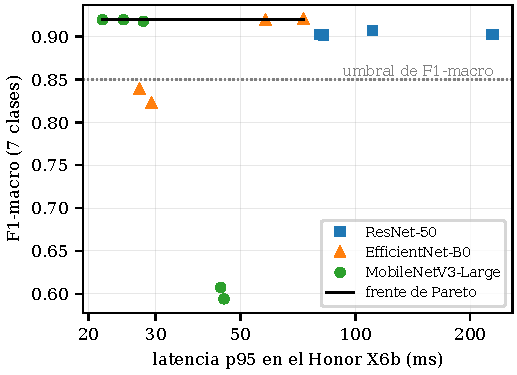
\includegraphics[width=\columnwidth]{fig/pareto.pdf}
\caption{F1-macro frente a la latencia p95 del modelo solo en el Honor X6b, para las tres arquitecturas en sus
cinco formatos.}
\label{fig:pareto}
\end{figure}

El prototipo con MobileNetV3-Large en float16, medido de extremo a extremo sobre 120 fotografías de locales de
prueba tal como las guarda ODK, tiene una mediana de 71~ms, un p95 de 110~ms y una memoria pico de 175~MB. Sobre
53 capturas a resolución completa de cámara, 108~ms, 159~ms y 233~MB. El modelo y el intérprete suman 10.0~MB.

\subsection{Verificación contra el convenio}

Las maestras alcanzan una parte de la prueba: 6\,035 de las 13\,972 fotografías son de un local con convenio
fechado, 61 de los 112 locales. De ellas, 5\,037 muestran un mueble de ese convenio o un rechazo, y 998, un mueble
que el convenio no lista. La exactitud condicionada al local que definía la planificación se mide sobre las
5\,037: 0.980 sin restringir y 0.986 con la predicción restringida.

\begin{table}[t]
\caption{Verificación con MobileNetV3-Large según la decisión}
\label{tab:decision}
\centering
\setlength{\tabcolsep}{3pt}
\begin{tabular}{@{}lccc@{}}
\toprule
Medida & Restringida & Sin restringir & Umbral \\
\midrule
Exactitud, 6\,035 con convenio & 0.823 & 0.974 & 0.974 \\
\midrule
\multicolumn{4}{@{}l}{\emph{Locales con un solo mueble contratado}} \\
Alerta ante otro mueble, de 333 & 161 & 333 & 333 \\
Falsas alarmas, de 243 & 3 & 13 & 13 \\
\midrule
\multicolumn{4}{@{}l}{\emph{Pares por intercambio}} \\
Falsas alarmas, 3\,333 correctos & 1.3\% & 1.6\% & 1.5\% \\
Detección, 5\,515 discrepantes & 99.3\% & 99.3\% & 99.3\% \\
Detección, fuera del convenio & 56.1\% & 98.8\% & 98.7\% \\
\midrule
\multicolumn{4}{@{}l}{\emph{Declaraciones reales de ODK}} \\
Falsas alarmas, 1\,075 correctas & 27.4\% & 3.0\% & 3.0\% \\
Errores detectados, de 73 & 72 & 65 & 67 \\
\bottomrule
\end{tabular}
\end{table}

La tabla~\ref{tab:decision} compara las tres decisiones de la sección~\ref{sec:decision}. La falla de la decisión
restringida es medible. En los 21
locales de prueba con un solo mueble contratado hay 333 fotografías que muestran otro mueble, y la decisión
restringida da el contratado en 172: si ese era el declarado, no hay alerta. Sobre las 998 fotografías de un
mueble que el convenio no lista no acierta nunca, por construcción, y su exactitud en las 6\,035 es 0.823. Con el
umbral calibrado en validación, $\tau = 0.47$, la exactitud sube a 0.974 y las 333 fotografías dan alerta. El
costo es que la restricción también tapaba errores del modelo: las falsas alarmas pasan de 1.3\% a 1.5\% en
los pares por intercambio, dentro del límite de 5\%, y de 3 a 13 de 243 fotografías (5.3\%) en los locales con
un solo mueble. El umbral casi no actúa: la red suele estar segura cuando ve un mueble fuera del convenio, y la
decisión coincide con la no restringida salvo en pocas fotografías.

Los dos experimentos responden preguntas distintas. Los pares por intercambio parten de 3\,333 fotografías de 45
locales y construyen 5\,515 discrepancias; la detección es de 99.3\%, pero en ellos la fotografía siempre
muestra un mueble contratado y bien tomado, declarado como otro. Las declaraciones reales de ODK son 1\,148
fotografías de 65 locales, de las que 73 (6.4\%) no muestran lo declarado: 58 muestran otro mueble, 12 contenido
ajeno y 3 son capturas inválidas. Con la decisión con umbral se detectan 67 (0.918, intervalo de Wilson
[0.832, 0.962]), con falsas alarmas en 32 de las 1\,075 correctas (3.0\%). La cifra de campo es esta última, y
su intervalo es ancho porque son 73 errores. La decisión restringida da 27.4\% de falsas alarmas sobre las
mismas fotografías, porque otros formularios declaran muebles ganados en negociación que la maestra no lista.

\subsection{Generalización temporal}

La prueba del experimento B son 1\,329 fotografías del último trimestre de 2025; no tiene capturas inválidas y
tiene tres de contenido ajeno. La tabla~\ref{tab:temporal} compara el modelo B con el modelo A sobre las mismas
fotografías. El modelo A, que entrenó con todo el periodo, no rinde mejor que el B, de modo que la baja frente al
periodo anterior no viene de haber entrenado solo con fotografías antiguas. Casi toda la baja es aritmética: la
clase de tres fotografías pesa un sexto del promedio y dos arquitecturas no aciertan ninguna. Sobre las cinco
clases de mueble, el F1-macro de B es 0.966 en MobileNetV3-Large, 0.958 en EfficientNet-B0 y 0.935 en ResNet-50.

\begin{table}[t]
\caption{Experimento B: F1-macro sobre las seis clases presentes en su prueba}
\label{tab:temporal}
\centering
\setlength{\tabcolsep}{3.5pt}
\begin{tabular}{@{}lccc@{}}
\toprule
Arquitectura & Modelo B & Modelo A & A $-$ B, IC 95\% \\
\midrule
ResNet-50 & 0.779 & 0.790 & $+0.010$ $[-0.008, +0.030]$ \\
EfficientNet-B0 & 0.846 & 0.836 & $-0.010$ $[-0.042, +0.019]$ \\
MobileNetV3-Large & 0.805 & 0.782 & $-0.023$ $[-0.040, -0.008]$ \\
\bottomrule
\end{tabular}
\end{table}

\subsection{Consistencia entre el teléfono y la evaluación}

El teléfono y la evaluación dan la misma clase en las 120 fotografías como las guarda ODK y en 51 de las 53
capturas a resolución de cámara. Para explicar las dos diferencias se repitió en Python el preprocesamiento del
teléfono, paso a paso, comparando cada variante con las probabilidades que dio el teléfono. La orientación no es
la causa: enderezar la fotografía antes o después de reducirla da los mismos resultados. El redimensionamiento
explica la mayor parte: la evaluación reduce con el filtro de Lanczos y el teléfono con mitades bilineales, y al
emular la reducción del teléfono la diferencia mediana de probabilidad baja de 0.024 a 0.007. Contribuye también
que la evaluación lee una copia recomprimida en JPEG y el teléfono no. Lo que queda no está explicado: la
emulación sigue a 0.007 del teléfono y no reproduce una de las dos diferencias. Que venga del decodificador JPEG o
del escalado de Android es una hipótesis que no se probó. Las dos fotografías son capturas inválidas en que el
modelo duda, con probabilidad máxima de 0.35; en una, el teléfono la acepta como mueble y la evaluación la rechaza.

Con esa emulación, que reproduce la clase del teléfono en 172 de las 173 fotografías medidas, se procesó toda la
prueba. Es una emulación y no una medición en el teléfono. La clase cambia en 80 de las 13\,972 fotografías
(0.57\%) y la decisión de aceptar o rechazar, en 15 (0.11\%), ninguna entre las 12\,787 en que el modelo da una
probabilidad de 0.9 o más. El recall de captura inválida es el mismo.

Esa cifra no mide las alertas. Aceptar o rechazar solo cambia cuando la fotografía pasa entre una categoría de
rechazo y una de mueble. La alerta compara la decisión con el mueble declarado, y cambia también cuando la
fotografía pasa de un mueble a otro o cuando su probabilidad cruza $\tau$. Sobre las 1\,148 fotografías de ODK con
un mueble declarado y la decisión con umbral, la alerta cambia en 3:
\begin{itemize}
\item una fotografía correcta deja de dar falsa alarma;
\item un error de campo pasa a detectarse;
\item otro error deja de detectarse.
\end{itemize}
Los errores detectados quedan en 67 de 73 y las falsas alarmas pasan de 32 a 31. La primera cifra mide cuánto
cambia el filtro de fotografías inservibles o ajenas; la segunda, cuánto cambia lo que ve quien verifica la
exhibición.

\subsection{Viabilidad}

Ninguna configuración es viable. En todas, el criterio que lo impide es el recall de captura inválida.
MobileNetV3-Large y EfficientNet-B0, en float32 y en float16, cumplen los otros ocho criterios, incluidos los del
dispositivo. ResNet-50 incumple además el recall-macro y el tamaño, y el int8 completo de las arquitecturas
eficientes incumple la degradación. Como preveía la regla, no se recomienda ninguna configuración.

\section{Conclusiones y trabajo futuro}

\textbf{Primera pregunta.} La arquitectura convencional no supera a las eficientes. ResNet-50 obtiene un F1-macro
de 0.903, frente a 0.920 de MobileNetV3-Large y 0.919 de EfficientNet-B0, y la diferencia no es significativa.
Pesa además más que el límite en todos sus formatos.

\textbf{Segunda pregunta.} La cuantización completa a int8 no es utilizable en las arquitecturas eficientes:
cuesta 0.325 de F1-macro en MobileNetV3-Large y 0.081 en EfficientNet-B0, contra un margen de 0.02. Reduce el
tamaño a cerca de la cuarta parte y la memoria a menos de la mitad. La latencia baja a menos de la mitad en
EfficientNet-B0 y en ResNet-50, pero se duplica en MobileNetV3-Large. La hipótesis sobre el int8 no se cumple. float16 conserva el desempeño con la mitad del tamaño y la misma
latencia; es una alternativa de despliegue, no una prueba de esa hipótesis.

\textbf{Tercera pregunta.} Ninguna configuración satisface todos los umbrales. Latencia, memoria y tamaño no son
el obstáculo: el teléfono de gama baja clasifica una fotografía en cerca de una décima de segundo. El obstáculo es reconocer
las capturas inválidas reales, que el modelo confunde con contenido ajeno o con un mueble cuando todavía se
distingue algo en la imagen.

El trabajo deja además dos resultados sobre la verificación. Restringir la decisión al convenio, como estaba
previsto, hace pasar por contratado un mueble que el convenio no lista. Conservar la predicción cuando hay
evidencia de otro mueble lo corrige en la prueba con un costo acotado en falsas alarmas. Como la corrección se
introdujo después de ver esa prueba, falta confirmarla con fotografías nuevas. Y la detección medida con discrepancias
construidas (99.3\%) sobreestima la de campo (67 de 73 errores reales).

\subsection{Limitaciones}

\textbf{Capturas inválidas.} Las 90 de la prueba son pocas, 62 son inducidas y provienen de 16 locales. El
resultado establece que el criterio no se cumple, no cuánto falta en producción.

\textbf{Decisión con umbral.} La regla se introdujo durante el análisis, después de identificar la falla en la
prueba. El umbral sale de la validación y no se reentrenó ningún modelo, pero la exactitud de 0.974 y las demás
cifras de la verificación con umbral son reproducibles, no independientes: su generalización debe confirmarse con
fotografías de campo nuevas que no hayan participado en el análisis.

\textbf{Cobertura de la verificación.} Las maestras cubren el 43\% de la prueba y no traen los muebles ganados
en negociación. Los errores reales de campo son 73.

\textbf{Etiquetas.} La auditoría encontró 4\% de desacuerdo en su muestra. Las capturas inválidas se auditaron
todas; en el resto de la prueba cabe esperar una proporción parecida de etiquetas discutibles.

\textbf{Dispositivo y prototipo.} Se midió un solo modelo de teléfono. La prueba del prototipo desde el formulario,
frente a muebles reales, fue de funcionamiento y con siete fotografías en un solo local. Con la decisión con
umbral, una cabecera fotografiada en un local que solo tiene check out dio la alerta de otro mueble (la decisión
restringida la habría aceptado), y una fotografía movida y otra del piso dieron la de fotografía inservible.

\textbf{Diagnóstico del int8.} Se hizo con fotografías de la prueba. Sirve para describir; si se buscara una
variante de int8 para usarla, la comparación tendría que hacerse con validación. Muestra que ninguna causa simple
basta por sí sola, pero no identifica la causa de la degradación.

\subsection{Trabajo futuro}

Lo primero es reunir capturas inválidas espontáneas, que el uso continuo de ODK produce cada
mes, para entrenar y para estimar el desempeño en producción. Lo segundo es sintetizar los defectos que hoy solo
existen en ejemplares reales: encuadres inclinados, al piso y al techo. Lo tercero es probar la decisión con umbral
en campo, con mercaderistas, y medir cuántas alertas llevan a repetir la fotografía. Quedan fuera de este trabajo
la extensión a farmacias y al canal tradicional, y la verificación de negocio y marca dentro del mueble.

\section*{Disponibilidad}

El código, los cuadernos con los resultados y la planificación están en
\url{https://github.com/sgarzong/tesis-ejecucion}. Las fotografías son de Industrias Ales y no se publican. Un
paquete de evidencias sin fotografías ni modelos (manifiestos, partición congelada, convenios, bitácoras de
etiquetado, predicciones y mediciones del teléfono) permite recalcular todas las cifras de este documento.

% Pendiente del autor: confirmar el texto de esta declaración con lo que pida el programa.
\section*{Uso de inteligencia artificial}

El código se escribió con asistencia de Claude Code (Anthropic), que también asistió en la redacción de este
documento. Las decisiones de diseño, el etiquetado y la interpretación de los resultados son del autor.

\begin{thebibliography}{99}

\bibitem{hartung2010odk} C. Hartung, A. Lerer, Y. Anokwa, C. Tseng, W. Brunette y G. Borriello, ``Open Data Kit:
Tools to build information services for developing regions,'' en \emph{Proc. 4th ACM/IEEE Int. Conf. Information
and Communication Technologies and Development (ICTD)}, 2010.

\bibitem{tonioni2018} A. Tonioni, E. Serra y L. Di Stefano, ``A deep learning pipeline for product recognition on
store shelves,'' arXiv:1810.01733, 2018.

\bibitem{wei2019rpc} X.-S. Wei, Q. Cui, L. Yang, P. Wang y L. Liu, ``RPC: A large-scale retail product checkout
dataset,'' arXiv:1901.07249, 2019.

\bibitem{goldman2019} E. Goldman, R. Herzig, A. Eisenschtat, J. Goldberger y T. Hassner, ``Precise detection in
densely packed scenes,'' en \emph{Proc. IEEE/CVF Conf. Computer Vision and Pattern Recognition (CVPR)}, 2019,
pp. 5227--5236.

\bibitem{peng2020rp2k} J. Peng, C. Xiao y Y. Li, ``RP2K: A large-scale retail product dataset for fine-grained
image classification,'' arXiv:2006.12634, 2020.

\bibitem{wei2020review} Y. Wei, S. N. Tran, S. Xu, B. Kang y M. Springer, ``Deep learning for retail product
recognition: Challenges and techniques,'' \emph{Computational Intelligence and Neuroscience}, vol. 2020, 2020.

\bibitem{sandler2018} M. Sandler, A. Howard, M. Zhu, A. Zhmoginov y L.-C. Chen, ``MobileNetV2: Inverted residuals
and linear bottlenecks,'' en \emph{Proc. IEEE Conf. Computer Vision and Pattern Recognition (CVPR)}, 2018,
pp. 4510--4520.

\bibitem{howard2019} A. Howard \emph{et al.}, ``Searching for MobileNetV3,'' en \emph{Proc. IEEE/CVF Int. Conf.
Computer Vision (ICCV)}, 2019, pp. 1314--1324.

\bibitem{tan2019} M. Tan y Q. V. Le, ``EfficientNet: Rethinking model scaling for convolutional neural
networks,'' en \emph{Proc. 36th Int. Conf. Machine Learning (ICML)}, 2019, pp. 6105--6114.

\bibitem{tan2021} M. Tan y Q. V. Le, ``EfficientNetV2: Smaller models and faster training,'' en \emph{Proc. 38th
Int. Conf. Machine Learning (ICML)}, 2021, pp. 10096--10106.

\bibitem{vasu2023} P. K. A. Vasu, J. Gabriel, J. Zhu, O. Tuzel y A. Ranjan, ``MobileOne: An improved one
millisecond mobile backbone,'' en \emph{Proc. IEEE/CVF Conf. Computer Vision and Pattern Recognition (CVPR)},
2023, pp. 7907--7917.

\bibitem{mehta2022} S. Mehta y M. Rastegari, ``MobileViT: Light-weight, general-purpose, and mobile-friendly
vision transformer,'' en \emph{Proc. Int. Conf. Learning Representations (ICLR)}, 2022.

\bibitem{qin2024} D. Qin \emph{et al.}, ``MobileNetV4: Universal models for the mobile ecosystem,'' en \emph{Proc.
European Conf. Computer Vision (ECCV)}, 2024.

\bibitem{jacob2018} B. Jacob \emph{et al.}, ``Quantization and training of neural networks for efficient
integer-arithmetic-only inference,'' en \emph{Proc. IEEE Conf. Computer Vision and Pattern Recognition (CVPR)},
2018, pp. 2704--2713.

\bibitem{gholami2021} A. Gholami, S. Kim, Z. Dong, Z. Yao, M. W. Mahoney y K. Keutzer, ``A survey of quantization
methods for efficient neural network inference,'' arXiv:2103.13630, 2021.

\bibitem{hinton2015} G. Hinton, O. Vinyals y J. Dean, ``Distilling the knowledge in a neural network,''
arXiv:1503.02531, 2015.

\bibitem{northcutt2021} C. G. Northcutt, L. Jiang e I. L. Chuang, ``Confident learning: Estimating uncertainty in
dataset labels,'' \emph{Journal of Artificial Intelligence Research}, vol. 70, pp. 1373--1411, 2021.

\bibitem{wilson1927} E. B. Wilson, ``Probable inference, the law of succession, and statistical inference,''
\emph{Journal of the American Statistical Association}, vol. 22, no. 158, pp. 209--212, 1927.

\bibitem{cohen1960} J. Cohen, ``A coefficient of agreement for nominal scales,'' \emph{Educational and
Psychological Measurement}, vol. 20, no. 1, pp. 37--46, 1960.

\bibitem{kapoor2023} S. Kapoor y A. Narayanan, ``Leakage and the reproducibility crisis in
machine-learning-based science,'' \emph{Patterns}, vol. 4, no. 9, 2023.

\bibitem{youden1950} W. J. Youden, ``Index for rating diagnostic tests,'' \emph{Cancer}, vol. 3, no. 1,
pp. 32--35, 1950.

\bibitem{deng2009} J. Deng, W. Dong, R. Socher, L.-J. Li, K. Li y L. Fei-Fei, ``ImageNet: A large-scale
hierarchical image database,'' en \emph{Proc. IEEE Conf. Computer Vision and Pattern Recognition (CVPR)}, 2009,
pp. 248--255.

\bibitem{he2016} K. He, X. Zhang, S. Ren y J. Sun, ``Deep residual learning for image recognition,'' en
\emph{Proc. IEEE Conf. Computer Vision and Pattern Recognition (CVPR)}, 2016, pp. 770--778.

\bibitem{tflite2022} TensorFlow, ``Post-training quantization,'' TensorFlow Model Optimization, 2022.

\bibitem{efron1979} B. Efron, ``Bootstrap methods: Another look at the jackknife,'' \emph{The Annals of
Statistics}, vol. 7, no. 1, pp. 1--26, 1979.

\end{thebibliography}

\end{document}
